\documentclass[12pt]{beamer}
%\includeonlyframes{current}

\mode<presentation>{\usetheme{Warsaw}}
\setbeamertemplate{footline}[frame number]
\usepackage[english]{babel}
\usepackage{times}
\usepackage{url}
\usepackage{graphicx}
\usepackage{hhline}
\usepackage{array}
\usepackage{colortbl}

\newcommand{\key}[1]{{\color{blue}#1}}
\newcommand{\cmnt}[1]{{\color{gray}#1}}
\newcommand{\str}[1]{{\color{green!50!black}#1}}
\newcommand{\num}[1]{{\color{green!55!blue}#1}}
\newcommand{\defn}[1]{{\color{purple}#1}}
\newcommand{\SC}[1]{\mbox{\sc#1}}
\newcommand{\EM}[1]{\mbox{\em#1}}
\newcommand{\tab}{\hspace{1em}}

\title{Statistical Learning Methods}
\subtitle{Introduction to Artificial Intelligence}
\author{Steven Bethard}
\institute{
  Department of Computer Science\\
  University of Colorado
}
\date{CSCI 3202}


\AtBeginSection[]{
\begin{frame}<beamer>{Outline}
	\tableofcontents[currentsection]
\end{frame}
}

\begin{document}

\begin{frame}
	\titlepage
\end{frame}

\begin{frame}{Outline}
	\tableofcontents
\end{frame}

\section{Naive Bayes}
\subsection{Models}
\begin{frame}{Naive Bayes Networks}
	\begin{columns}[t]
		\begin{column}{2in}
			\begin{block}{Bayesian Network}
				Represents all variable dependence relations
			\end{block}
			\begin{center}
				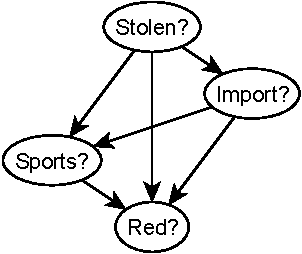
\includegraphics[scale=.75]{stolen-bayes-net}
			\end{center}
		\end{column}
		\pause
		\begin{column}{2in}
			\begin{block}{Naive Bayes Network}
				Assumes features are conditionally independent given the class variable
			\end{block}
			\begin{center}
				\includegraphics[scale=.75]{stolen-naive-bayes}
			\end{center}
		\end{column}
	\end{columns}
\end{frame}
\begin{frame}{Naive Bayes Models}
	\begin{block}{Given class variable $C$ and feature variables $F_1,\ldots,F_n$}
		$
		\begin{array}{llll}
			\lefteqn{\mathbf{P}(C|F_1,F_2,\ldots,F_n)} \\
			& = & \pause\alpha\mathbf{P}(F_1,F_2,\ldots,F_n|C)\mathbf{P}(C) & \mbox{Bayes' Rule} \\
			& = & \pause\alpha\mathbf{P}(F_1|C)\mathbf{P}(F_2|C)\ldots\mathbf{P}(F_n|C)\mathbf{P}(C) & \mbox{Naive Bayes}
		\end{array}
		$
	\end{block}
	\pause
	\vspace{-1pt}
	\begin{block}{Naive Bayes models}
		$\mathbf{P}(C|F_1,F_2,\ldots,F_n) = \alpha\mathbf{P}(C)\prod\limits_{i=1}^{n}\mathbf{P}(F_{i}|C)$
	\end{block}
	\pause
	\vspace{-1pt}
	\begin{block}{Training models}
		\begin{itemize}
			\item Find the probability of each class
			\item Find the probability of each feature given the class
		\end{itemize}
	\end{block}
\end{frame}


\subsection{Examples}
\begin{frame}{Naive Bayes Classification}
	\centering
	\begin{tabular}[t]{lll|l}
		Origin?  & Color? & Type?  & Stolen? \\
		\hline
		import   & red    & sports & yes \\
		import   & red    & sports & yes \\
		domestic & white  & sports & yes \\
		domestic & red    & van    & yes \\
		import   & red    & van    & no \\
		domestic & white  & sports & no \\
	\end{tabular}
	
	\pause
	\begin{block}{A domestic red sports car}
	\small
	$
	\begin{array}{@{}l@{\hspace{.1em}}l@{\hspace{.1em}}l@{\hspace{.1em}}l@{\hspace{.1em}}l@{\hspace{.1em}}l@{\hspace{.1em}}l@{}}
		\pause
		P(y|d,r,s) & = & \pause\alpha P(y)P(d|y)P(r|y)P(s|y) 
		           & = & \pause\alpha\cdot\pause\frac{2}{3}\cdot\pause\frac{1}{2}\cdot\pause\frac{3}{4}\cdot\pause\frac{3}{4}
		           & = & \pause\frac{3}{16}\alpha
		\\
		\pause
		P(n|d,r,s) & = & \pause\alpha P(n)P(d|n)P(r|n)P(s|n)
		           & = & \pause\alpha\cdot\frac{1}{3}\cdot\frac{1}{2}\cdot\frac{1}{2}\cdot\frac{1}{2}
		           & = & \pause\frac{1}{24}\alpha
	\end{array}
	$
	\normalsize
	\medskip
	
	\pause
	Predict stolen?
	\pause
	\alert{yes}
	\hfill
	\pause
	At what probability?
	\pause
	$\alert{\frac{9}{11}} = \frac{\frac{3}{16}}{\frac{3}{16} + \frac{1}{24}}$
	\end{block}
\end{frame}
\begin{frame}{Naive Bayes Exercise}
	\begin{center}
		\begin{tabular}[t]{cc|c}
			Ends with -ed  & Initial Capital  & Part of Speech \\
			\hline
			no             & no               & noun \\
			no             & yes              & noun \\
			no             & yes              & noun \\
			yes            & no               & noun \\
			yes            & yes              & noun \\
			no             & no               & verb \\
			yes            & no               & verb \\
			yes            & yes              & verb \\
		\end{tabular}
		
		\bigskip
		Assign part of speech tags:
		\tab\tab
		\begin{tabular}[t]{cc}
			John            & tripped \\
			\pause
			noun            & verb    \\
			\pause
			.84375          & .625 \\
		\end{tabular}
	\end{center}
\end{frame}

\subsection{Properties}
\begin{frame}[<+->]{Naive Bayes Properties}
	\begin{block}{Naive Bayes assumption is hardly ever true}
		\begin{itemize}
			\item Probability estimates of Naive Bayes are poor
			\item Classification decisions are often surprisingly good
		\end{itemize}
	\end{block}
	\begin{block}{Empirical Observations}
		\begin{itemize}
			\item Works best when many equally important features
			\item Somewhat robust to noise (uninformative) features
			\item Training and classification are typically fast
		\end{itemize}
	\end{block}
\end{frame}

\section{k-Nearest Neighbor}
\subsection{Models}
\begin{frame}{k-Nearest Neighbor Basics}
	\begin{block}{Examples as Points}
		\begin{itemize}
			\item Treat examples as points in an $n$-dimensional space
			\item Each dimension corresponds to one feature
		\end{itemize}
	\end{block}
	\pause
	\begin{block}{k-Nearest Neighbor Algorithm}
		To classify a new example, $p$:
		\begin{itemize}
			\item Find the $k$ points closest to $p$
			\item Classify $p$ with the most common class
		\end{itemize}
	\end{block}
\end{frame}
\begin{frame}{1-Nearest Neighbor}
	\begin{center}
		\only<1>{\includegraphics[scale=.75]{knn-points}}%
		\only<2>{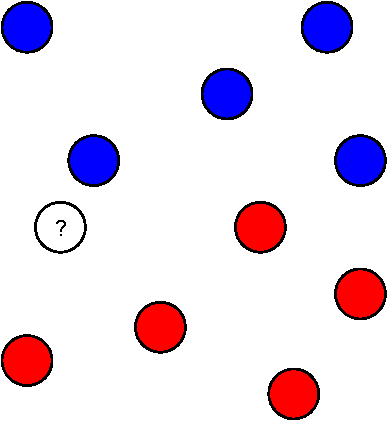
\includegraphics[scale=.75]{knn-test-point}}%
		\only<3>{\includegraphics[scale=.75]{knn-test-point-k1-1}}%
		\only<4>{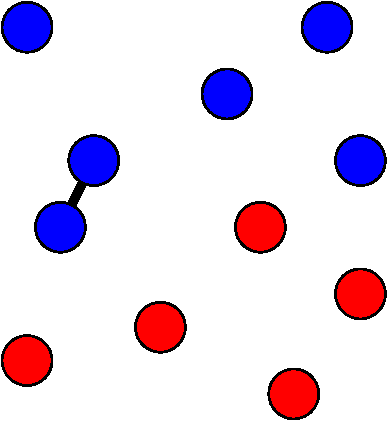
\includegraphics[scale=.75]{knn-test-point-k1-2}}%
	\end{center}
\end{frame}
\begin{frame}{3-Nearest Neighbor}
	\begin{center}
		\only<1>{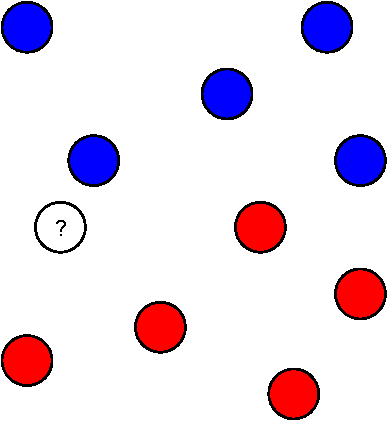
\includegraphics[scale=.75]{knn-test-point}}%
		\only<2>{\includegraphics[scale=.75]{knn-test-point-k3-1}}%
		\only<3>{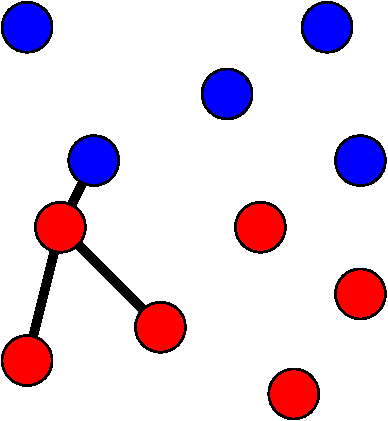
\includegraphics[scale=.75]{knn-test-point-k3-2}}%
	\end{center}
\end{frame}


\subsection{Distance}
\begin{frame}{Distance Metrics}
	\begin{columns}[T]
		\begin{column}{2in}
			\begin{block}{Euclidean Distance}
				$\sqrt{\sum\limits_{i=1}^{n}(a_i - b_i)^{2}}$
				\hfill
				\begin{tabular}{@{}l@{\hspace{.2em}}c@{}}
					close & 0 \\
					far   & $\infty$
				\end{tabular}
			\end{block}
		\end{column}
		\begin{column}{2in}
			\begin{block}{Cosine Distance}
				$
			  \displaystyle
			  \frac{\sum\limits_{i=1}^{n}a_i b_i}
			       {\sqrt{\sum\limits_{i=1}^{n}a_i^2}
			        \sqrt{\sum\limits_{i=1}^{n}b_i^2}}
				$
				\hfill
				\begin{tabular}{@{}l@{\hspace{.2em}}c@{}}
						close & 1 \\
						far   & -1
				\end{tabular}
			\end{block}
		\end{column}
	\end{columns}
	\bigskip
	\begin{columns}[T]
		\begin{column}{2in}
			\only<2>{\includegraphics[width=2in]{knn-distance}}%
			\only<3>{\includegraphics[width=2in]{knn-distance-euclidean-1}}%
			\only<4->{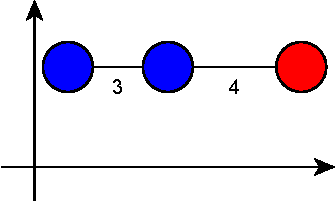
\includegraphics[width=2in]{knn-distance-euclidean-2}}%
		\end{column}
		\begin{column}{2in}
			\only<-4>{\invisible{\includegraphics[width=2in]{knn-distance}}}%
			\only<5>{\includegraphics[width=2in]{knn-distance}}%
			\only<6>{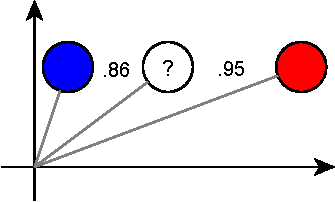
\includegraphics[width=2in]{knn-distance-cosine-1}}%
			\only<7->{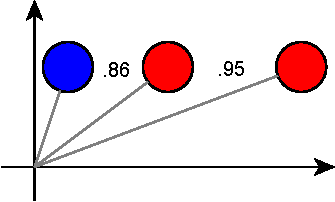
\includegraphics[width=2in]{knn-distance-cosine-2}}%
		\end{column}
	\end{columns}
\end{frame}
\begin{frame}{k-Nearest Neighbor Exercise}
	\begin{columns}[T]
		\begin{column}{2in}
			Training data:
			
			$
			\begin{array}{cc|c}
				F_0 & F_1 & C \\
				\hline
				-1  & 1   & A \\
				0   & 1   & A \\
				0   & 2   & A \\
				2   & 2   & B \\
				3   & 2   & B \\
				3   & 3   & B \\
			\end{array}
			$
	
			\smallskip
			Classify $(1, 1)$ with 3-NN
			\smallskip
			
			\small
			\begin{columns}
				\begin{column}{.9in}
					Euclidean: \uncover<2->{$A$
					
					$
					\begin{array}{cc|c@{}}
						0   & 1   & A \\
						0   & 2   & A \\
						2   & 2   & B \\
					\end{array}
					$}
				\end{column}
				\begin{column}{.7in}
					Cosine: \uncover<2->{$B$
					
					$
					\begin{array}{cc|c@{}}
						2   & 2   & B \\
						3   & 2   & B \\
						3   & 3   & B \\
					\end{array}
					$}
				\end{column}
			\end{columns}
		\end{column}
		\begin{column}{2in}
			\begin{block}{Euclidean Distance}
				$\sqrt{\sum\limits_{i=1}^{n}(a_i - b_i)^{2}}$
				\hfill
				\begin{tabular}{@{}l@{\hspace{.2em}}c@{}}
					close & 0 \\
					far   & $\infty$
				\end{tabular}
			\end{block}
			\begin{block}{Cosine Distance}
				$
			  \displaystyle
			  \frac{\sum\limits_{i=1}^{n}a_i b_i}
			       {\sqrt{\sum\limits_{i=1}^{n}a_i^2}
			        \sqrt{\sum\limits_{i=1}^{n}b_i^2}}
				$
				\hfill
				\begin{tabular}{@{}l@{\hspace{.2em}}c@{}}
						close & 1 \\
						far   & -1
				\end{tabular}
			\end{block}
		\end{column}
	\end{columns}
\end{frame}


\subsection{Properties}
\begin{frame}[<+->]{k-Nearest Neighbor Properties}
	\begin{block}{Theoretical Properties}
		\begin{itemize}
			\item Given enough data and the right $k$, minimizes error
			\item Able to approximate many kinds of functions
		\end{itemize}
	\end{block}
	\begin{block}{Empirical Issues}
		\begin{itemize}
			\item Simple to implement given a distance function
			\item Large training data means long search times
			\item Not always clear what distance function to use
		\end{itemize}
	\end{block}
\end{frame}


\section{Advanced Algorithms}
\subsection{Support Vector Machines}
\begin{frame}{Classification Hyperplanes}
	\begin{center}
		\only<1>{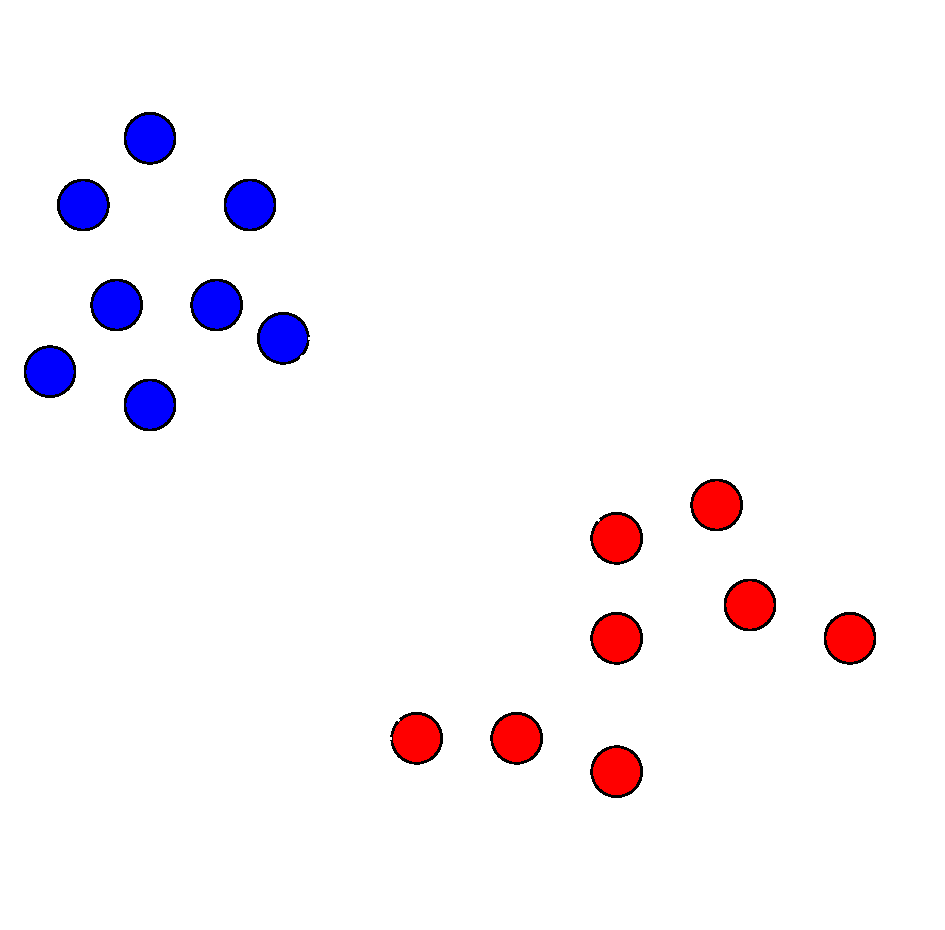
\includegraphics[height=2.7in]{hyperplanes-0}}%
		\only<2>{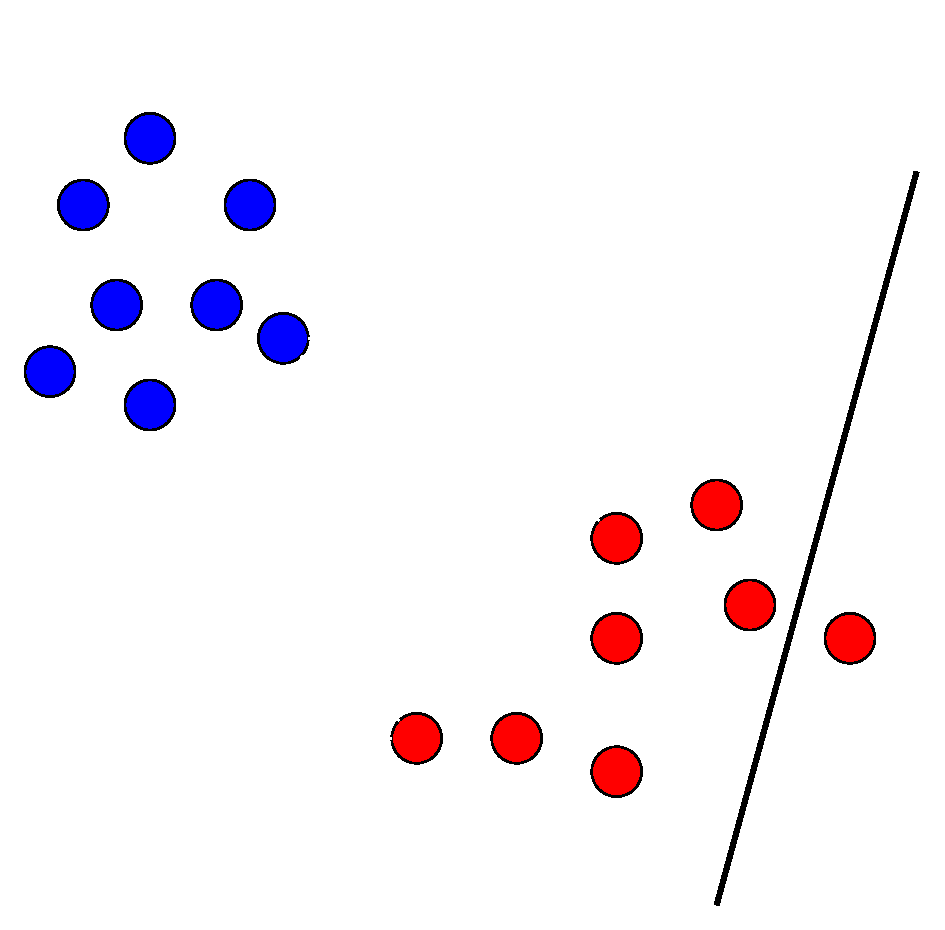
\includegraphics[height=2.7in]{hyperplanes-1}}%
		\only<3>{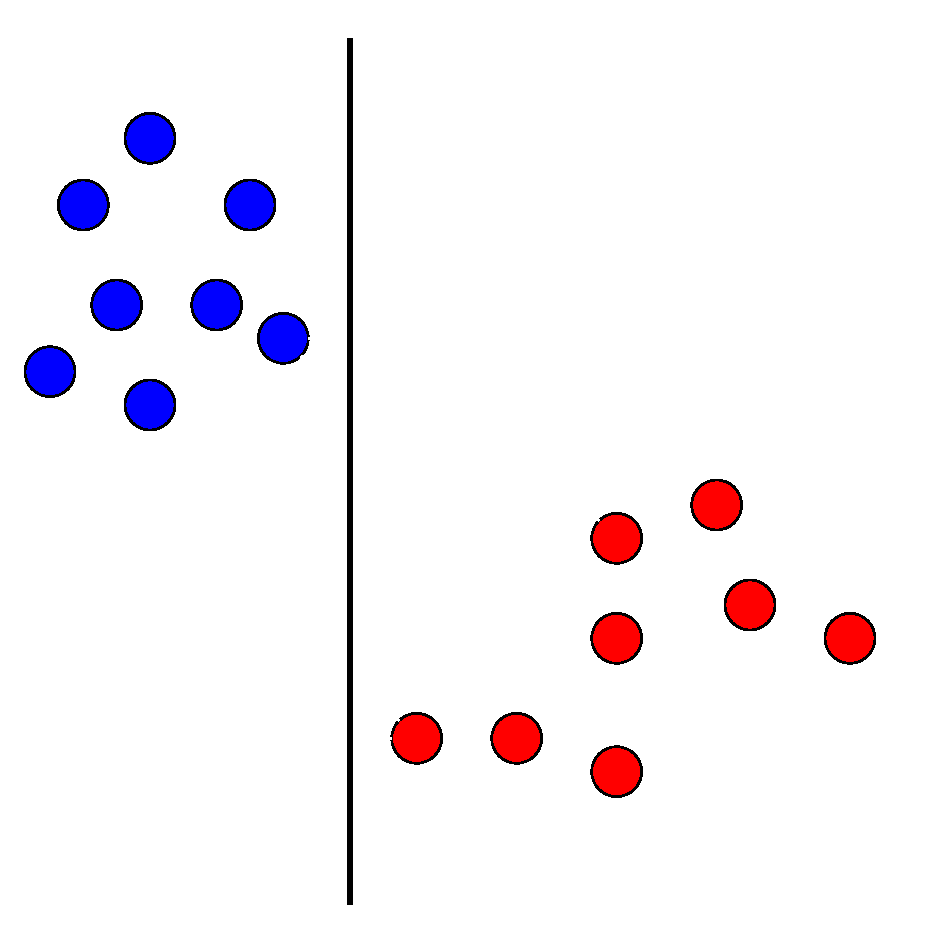
\includegraphics[height=2.7in]{hyperplanes-2}}%
		\only<4>{\includegraphics[height=2.7in]{hyperplanes-3}}%
	\end{center}
\end{frame}
\begin{frame}{Maximizing Margins}
	\begin{center}
		\only<1>{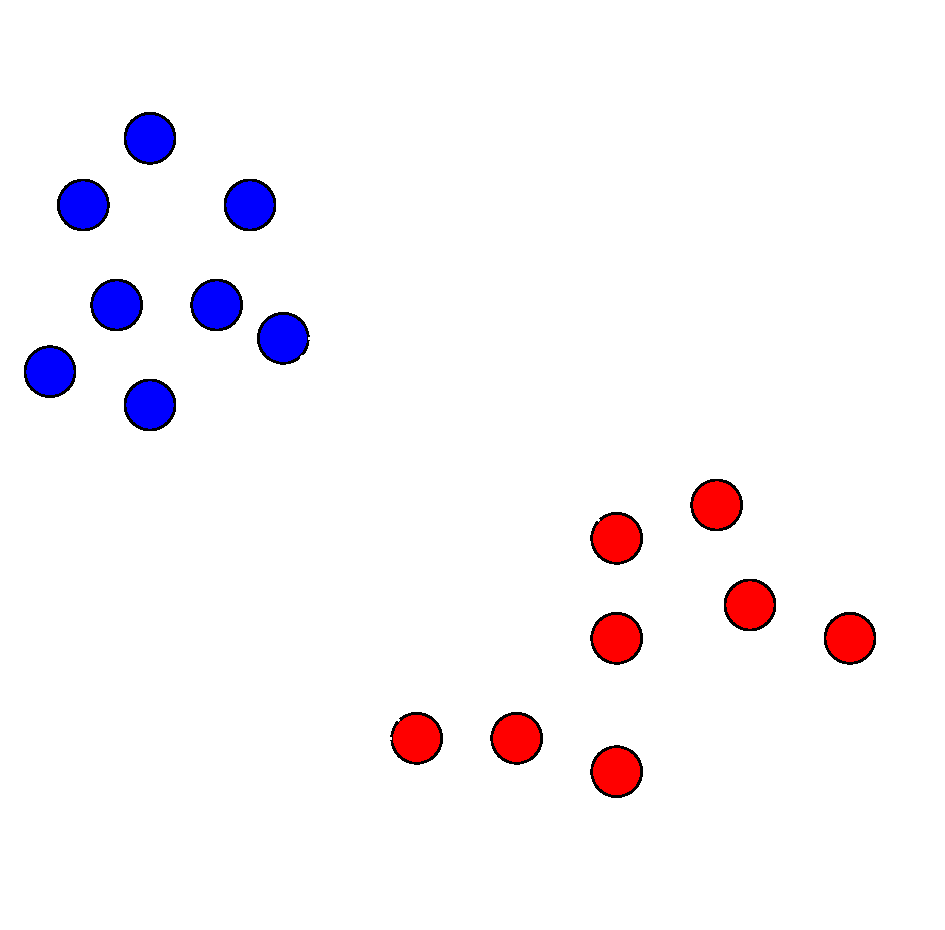
\includegraphics[height=2.7in]{hyperplanes-0}}%
		\only<2>{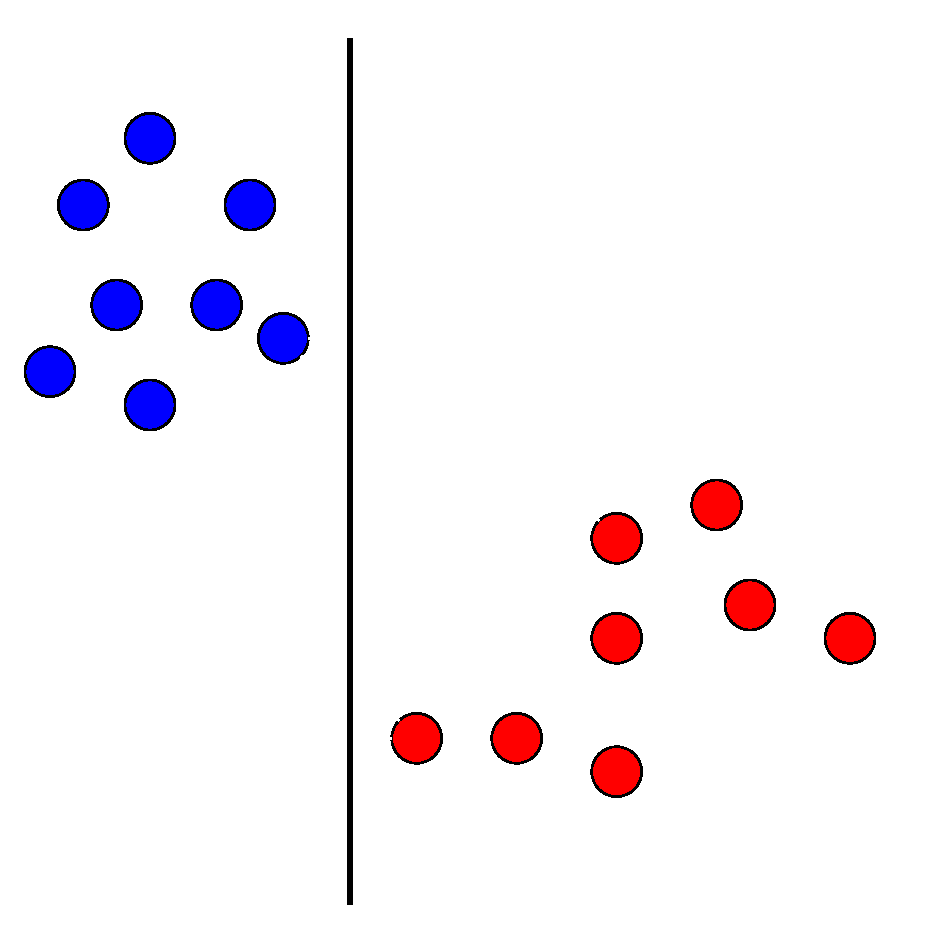
\includegraphics[height=2.7in]{hyperplanes-2}}%
		\only<3>{\includegraphics[height=2.7in]{hyperplanes-2-margins}}%
		\only<4>{\includegraphics[height=2.7in]{hyperplanes-3}}%
		\only<5>{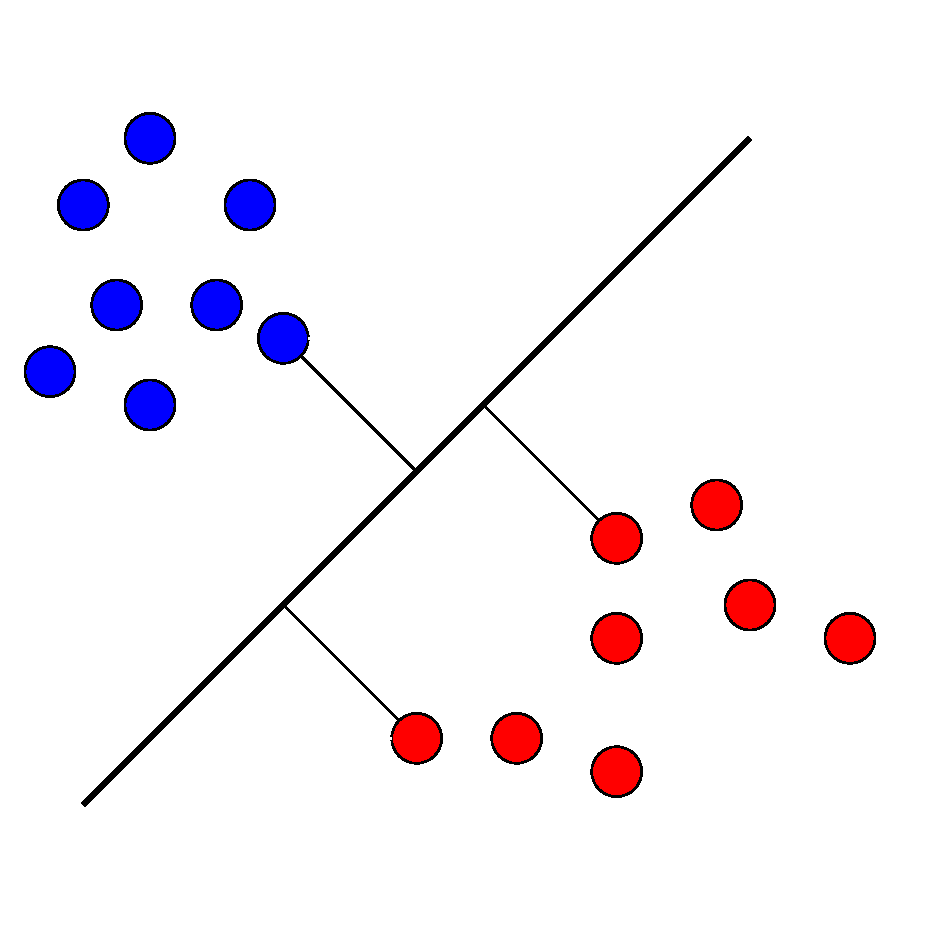
\includegraphics[height=2.7in]{hyperplanes-3-margins}}%
	\end{center}
\end{frame}
\begin{frame}{Identifying Support Vectors}
	\begin{center}
		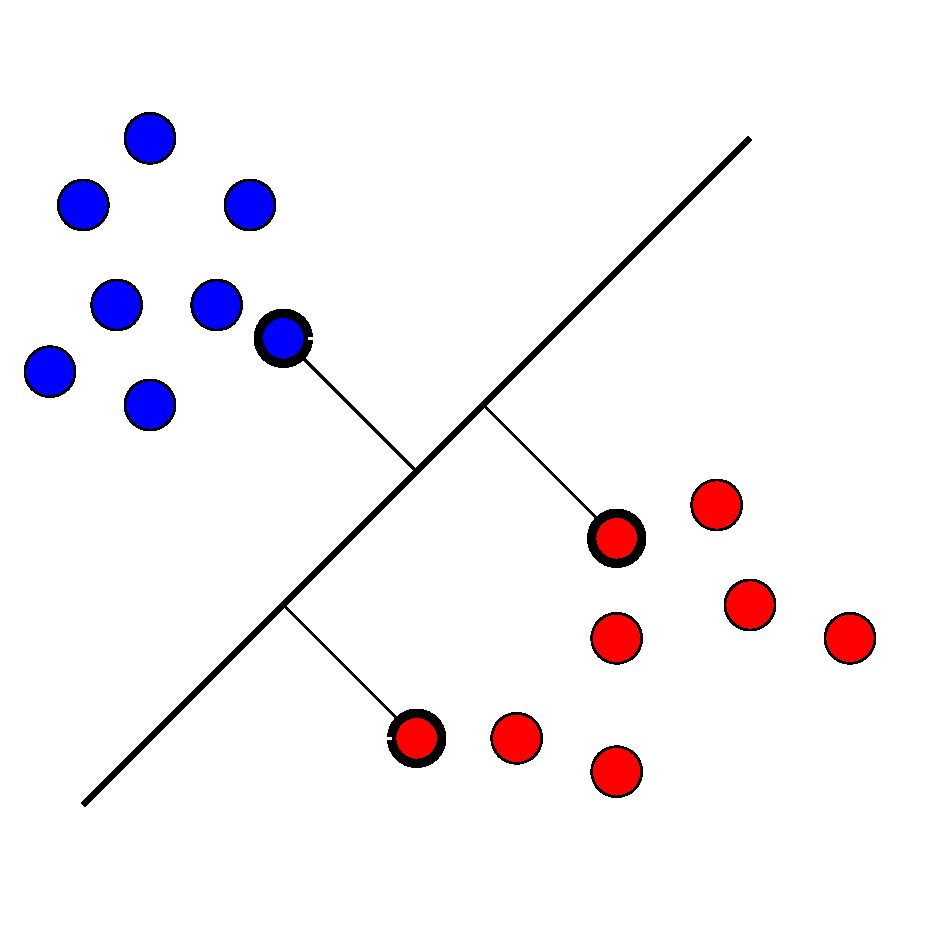
\includegraphics[height=2.7in]{hyperplanes-3-support-vectors}%
	\end{center}
\end{frame}
\begin{frame}{Support Vector Machines}
	\begin{block}{Key Ideas}
		\begin{itemize}
			\item Maximize the margin of the separating hyperplane
			\item Only support vectors needed for classification
		\end{itemize}
	\end{block}
	\begin{block}{Calculating the Maximum Margin}
		\begin{itemize}
			\item Requires a quadratic programming optimization
			\item Heuristics and approximations used to speed it up
		\end{itemize}
	\end{block}
\end{frame}
\begin{frame}{Nonlinear Classification with SVMs}
	\begin{columns}
		\begin{column}{2in}
			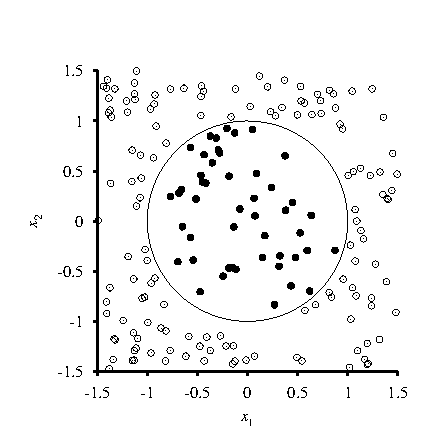
\includegraphics[height=1.55in]{svm-kernel-1}
			\\ \bigskip
			\centering
			Features: $(x_1, x_2)$ \\
			\alert{Not linearly separable}
		\end{column}
		\pause
		\begin{column}{2in}
			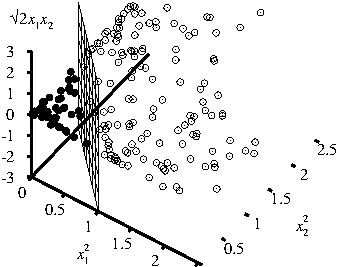
\includegraphics[height=1.55in]{svm-kernel-2}
			\\ \bigskip
			\centering
			Features: $(x_1, x_2, \sqrt{2} x_1 x_2)$ \\
			\alert{Linearly separable}
		\end{column}
	\end{columns}
\end{frame}
\begin{frame}{Kernel Methods}
	\begin{block}{Mapping features to higher dimensional spaces}
		\begin{itemize}
			\pause
			\item Allow linear classifiers to learn nonlinear functions
			\pause
			\item Works with any classifier, not just SVMs
			\pause
			\item \alert{But computing transformations is expensive}
		\end{itemize}
	\end{block}
	\pause
	\begin{block}{Kernel Trick}
		\begin{itemize}
			\pause
			\item Select kernel function $K(\mathbf{x}_{i}, \mathbf{x}_{j}) = \varphi(\mathbf{x}_{i}) \cdot \varphi(\mathbf{x}_{j})$
			\pause
			\item Replace dot product
				\begin{tabular}{ll}
					Linear SVM:
					& 
					$h(\mathbf{x}) = \mbox{sign}\left(\sum\limits_{i}\alpha_{i}y_{i}(\mathbf{x}\cdot\mathbf{x}_{i})\right)$
					\pause \\
					Kernel SVM:
					&
					$h(\mathbf{x}) = \mbox{sign}\left(\sum\limits_{i}\alpha_{i}y_{i}K(\mathbf{x},\mathbf{x}_{i})\right)$
				\end{tabular}
		\end{itemize}
	\end{block}
\end{frame}
\begin{frame}[<+->]{Support Vector Machine Properties}
	\begin{block}{Theoretical Properties}
		\begin{itemize}
			\item Efficient optimal separators in huge feature spaces
			\item Can approximate essentially any function
		\end{itemize}
	\end{block}
	\begin{block}{Empirical Issues}
		\begin{itemize}
			\item Classification usually fast, but training often slow
			\item Kernel functions (and parameters) chosen empirically
		\end{itemize}
	\end{block}
\end{frame}
\begin{frame}[fragile]{Support Vector Machine Demo}
	\begin{center}
		\small\url{http://www.csie.ntu.edu.tw/~cjlin/libsvm/#GUI}
	\end{center}
\end{frame}


\subsection{Neural Networks}
\begin{frame}{Neurons in the Brain}
	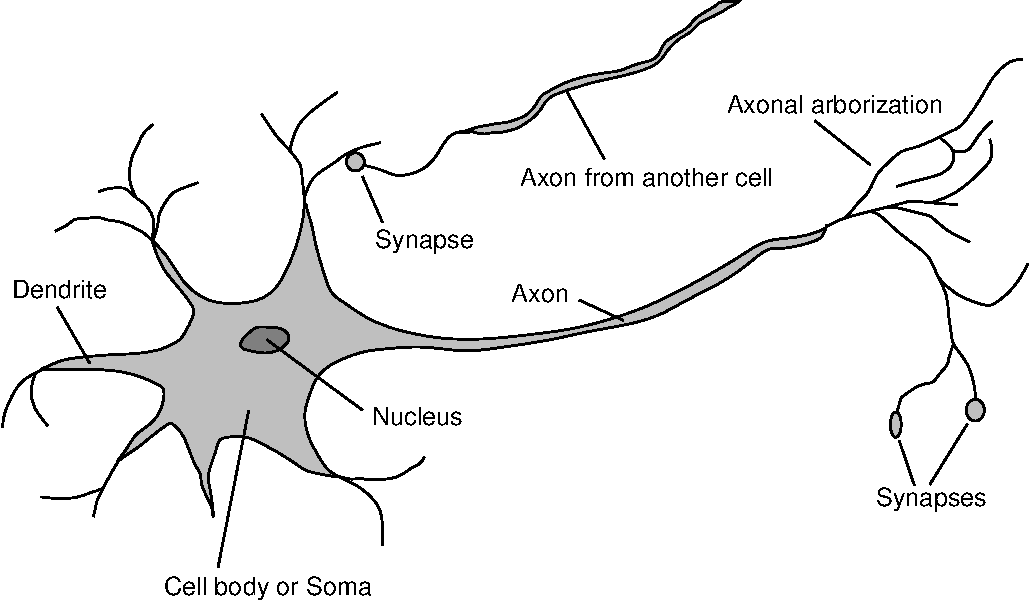
\includegraphics[width=4in]{neuron}
\end{frame}
\begin{frame}{Mathematical Model of a Neuron}
	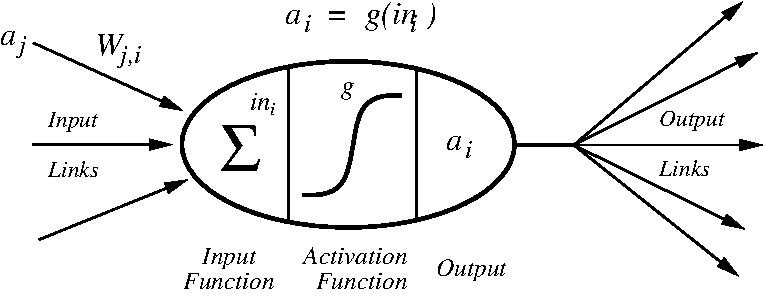
\includegraphics[width=4in]{neuron-unit}
\end{frame}
\begin{frame}{Neural Net Units}
	\begin{columns}
		\begin{column}{2.2in}
			\begin{block}{Unit computation}
				\centering
				$\displaystyle a_j = g\left(\sum\limits_{i}{W_{i,j} \cdot a_{i}}\right)$
			\end{block}
			\bigskip
			\begin{block}<2->{Activation functions}
				\begin{tabular}{ll@{}}
					\uncover<3->{Threshold & $\displaystyle g(x) = x > 0$ \\}
					\uncover<4->{Sigmoid   & $\displaystyle g(x) = \frac{1}{1 + e^{-x}}$}
				\end{tabular}
			\end{block}
		\end{column}
		\begin{column}<5->{2in}
			Logical ``and'' unit \\
			(threshold activation) \\
			\bigskip
			\only<-5>{ \includegraphics[height=1.25in]{neural-net-logical-and}}%
			\only<6>{  \includegraphics[height=1.25in]{neural-net-logical-and-1-1}}%
			\only<7>{  \includegraphics[height=1.25in]{neural-net-logical-and-1-2}}%
			\only<8>{  \includegraphics[height=1.25in]{neural-net-logical-and-1-3}}%
			\only<9>{  \includegraphics[height=1.25in]{neural-net-logical-and-1-4}}%
			\only<10>{ \includegraphics[height=1.25in]{neural-net-logical-and}}%
			\only<11>{ \includegraphics[height=1.25in]{neural-net-logical-and-2-1}}%
			\only<12>{ 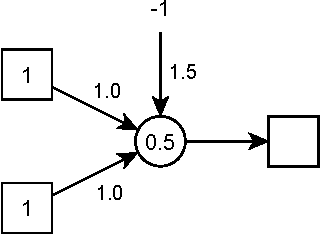
\includegraphics[height=1.25in]{neural-net-logical-and-2-2}}%
			\only<13>{ \includegraphics[height=1.25in]{neural-net-logical-and-2-3}}%
			\only<14->{\includegraphics[height=1.25in]{neural-net-logical-and-2-4}}%
		\end{column}
	\end{columns}
	\bigskip
	\uncover<15->{
	Interactive Demo: \\
	\footnotesize
	\url{http://lcn.epfl.ch/tutorial/french/aneuron/html/}}
\end{frame}
\begin{frame}{Neural Net Classification}
	\begin{center}
		Sum inputs, apply activation function, repeat
	\end{center}
	\begin{center}
		\only<1>{\includegraphics[height=2in]{neural-net-forward}}%
		\only<2>{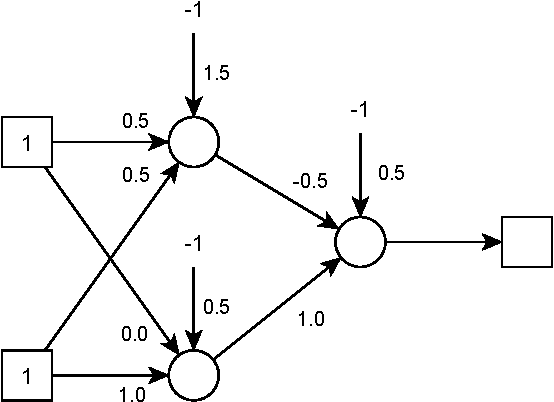
\includegraphics[height=2in]{neural-net-forward-1}}%
		\only<3>{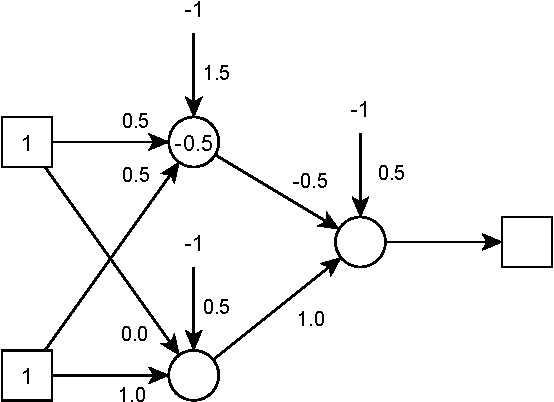
\includegraphics[height=2in]{neural-net-forward-2}}%
		\only<4>{\includegraphics[height=2in]{neural-net-forward-3}}%
		\only<5>{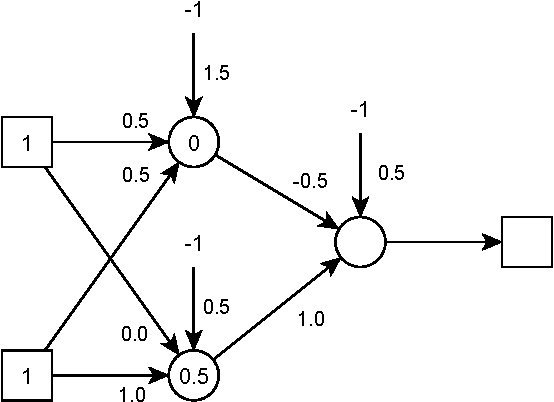
\includegraphics[height=2in]{neural-net-forward-4}}%
		\only<6>{\includegraphics[height=2in]{neural-net-forward-5}}%
		\only<7>{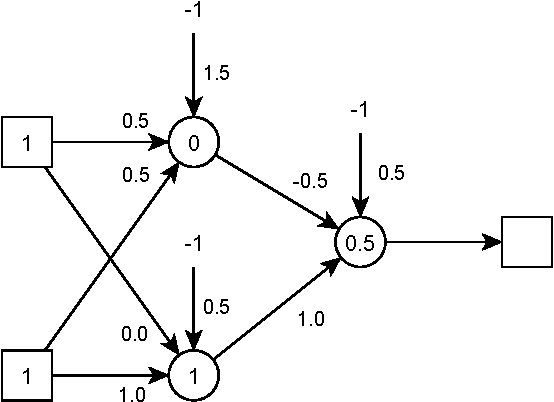
\includegraphics[height=2in]{neural-net-forward-6}}%
		\only<8>{\includegraphics[height=2in]{neural-net-forward-7}}%
		\only<9>{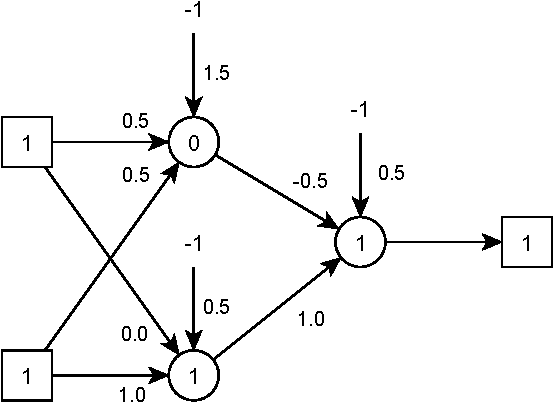
\includegraphics[height=2in]{neural-net-forward-8}}%
	\end{center}
\end{frame}
\begin{frame}{Neural Net Classification Exercise}
	\begin{center}
		\begin{itemize}
			\item Classify the input using the neural net
			\item Use threshold activation function
		\end{itemize}
	\end{center}
	\begin{center}
		\only<1>{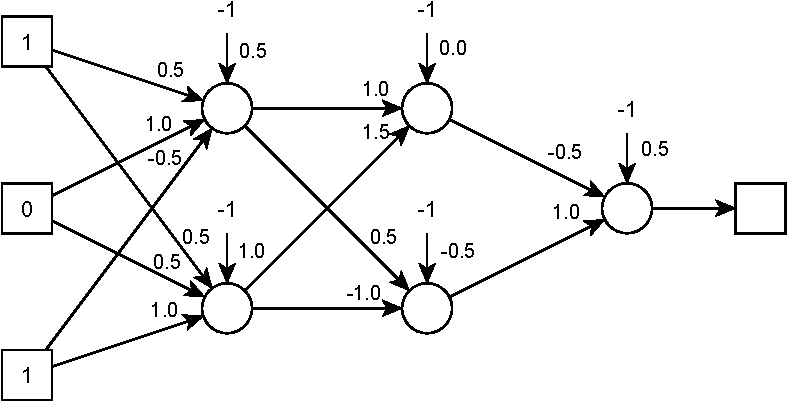
\includegraphics[height=2in]{neural-net-example}}%
		\only<2>{\includegraphics[height=2in]{neural-net-example-solution}}%
	\end{center}
\end{frame}
\begin{frame}[<+->]{Learning Neural Nets}
	\begin{block}{Back Propagation}
		\begin{itemize}
			\item Provide inputs and run network
			\item Compare network outputs to expected outputs
			\item Determine error for output units
			\item Propagate error back to earlier units
			\item Adjust weights to reduce errors
		\end{itemize}
	\end{block}
	\begin{block}{Back Propagation Properties}
		\begin{itemize}
			\item A gradient descent algorithm
			\item Can get stuck in local minima
		\end{itemize}
	\end{block}
\end{frame}
\begin{frame}[<+->]{Neural Net Properties}
	\begin{block}{Expressive Power}
		\begin{itemize}
			\item Single layer networks: linearly separable functions
			\item Multi-layer networks: essentially any function
		\end{itemize}
	\end{block}
	\begin{block}{Empirical Issues}
		\begin{itemize}
			\item How many hidden layers?
			\item How many nodes in each layer?
			\item How to initialize weights?
		\end{itemize}
	\end{block}
\end{frame}
\begin{frame}[fragile]{Neural Network Demo}
	\begin{center}
		\url{http://www.c2i.ntu.edu.sg/Courses/AI/CIspace/Version4/neural/}
	\end{center}
\end{frame}


\part{Key Ideas}
\begin{frame}{Key Ideas}
	\begin{block}{Naive Bayes}
		Assume features conditionally independent given class
	\end{block}
	\begin{block}{k-Nearest Neighbor}
		Use distance metric to find classes of closest examples
	\end{block}
	\begin{block}{Support Vector Machines}
		Find max margin separating hyperplane in kernel space
	\end{block}
	\begin{block}{Neural Networks}
		Sum inputs, apply activation function, repeat
	\end{block}
\end{frame}

\end{document}


